\classheader{10-09-2017}

\definition{A topological space $X$ is \textbf{locally connected} at $x$ if every open set $U$ containing $x$ has the property that there exists a $V\subseteq U$ such that $x\in V$, $V$ is open, and $V$ is connected.}

\definition{A topological space is \textbf{locally path connected} at $x$ if every open set $U$ containing $x$ has the property that there exists a $V\subseteq U$ such that $x\in V$, $V$ is open, and $V$ is path connected.}

\example{The topologist's interval is the subset of $\R^2$ defined piecewise as the union of the closed horizontal segment $[-1,0]$ along the $x$-axis, the closed vertical segment $[-1,1]$ along the $y$-axis, and the function $y=\sin(\frac{\pi}{x})$ on the interval $x\in (0,1]$. We give this the subspace topology from $\R^2$.
	
	
	\begin{figure}[!htb]
		\centering
		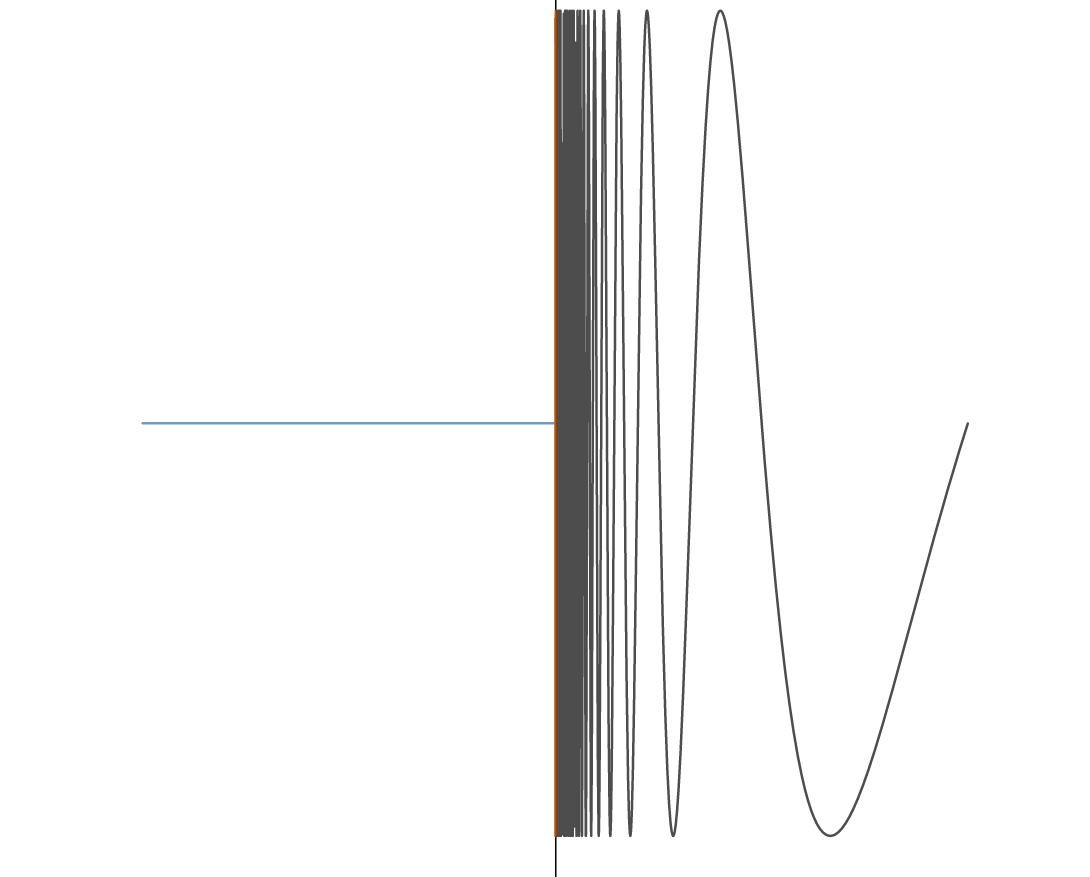
\includegraphics[scale=.2]{images/topint}
		\caption{The Topologist's Interval}
		\label{fig:topint}
	\end{figure}
	
	
	This space is connected, but not path connected, as the vertical stripes become infinitely close near zero, so there is no proper path from a point to the left of the origin to a point to the right.
	
	
	The topologist's circle is the same thing, but with an arc adjoined from $(1,0)$ to $(-1,0)$.
	
	\begin{figure}[!htb]
		\centering
		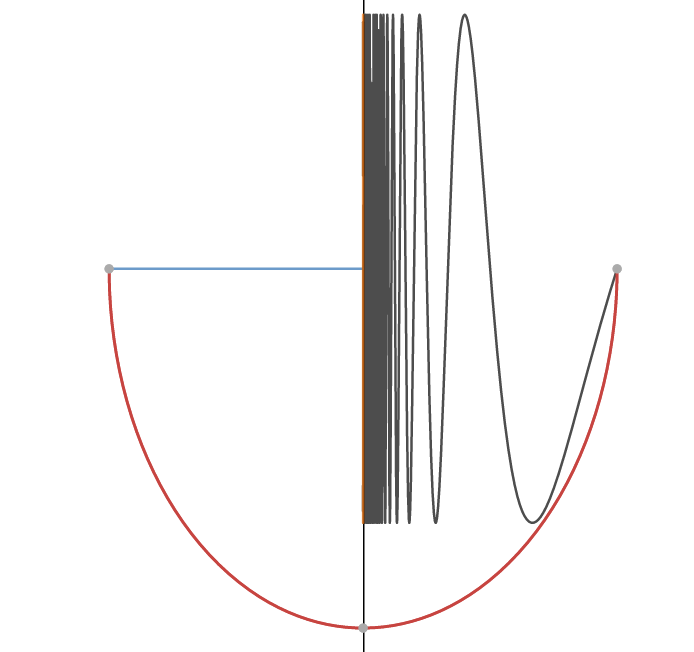
\includegraphics[scale=.3]{images/topcirc}
		\caption{The Topologist's Circle}
		\label{fig:topcirc}
	\end{figure}
	
	This space is connected and path connected, as we can use the arc to avoid the messiness to the right of the origin, but it is not locally path connected, as we can still look at small neighborhoods which look like parallel stripes, and obviously are not path connected.



The subset of $\R^2$ defined piecewise as the union of the closed horizontal segment $[-1,0]$ along the $x$-axis and $y=x\sin(\frac{\pi}{x})$ is locally connected everywhere, but not locally path connected at the origin.


	
	\begin{figure}[!htb]
		\centering
		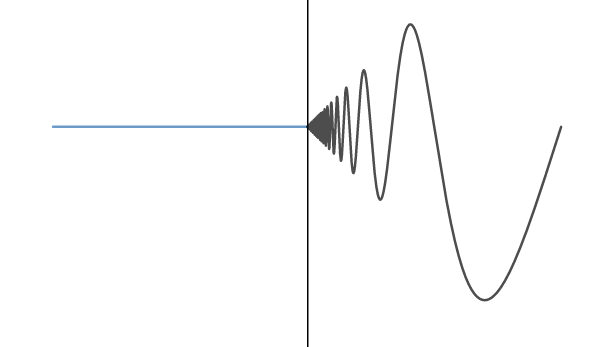
\includegraphics[scale=.3]{images/xsinx}
		\caption{$y=x\sin{\pi/x}$}
		\label{fig:xsinx}
	\end{figure}

}

\thrm{If a space $X$ is path connected, then it is connected.}

\begin{proof}
	
	Let $X$ be a path connected topological space.  If $X$ is not connected, then there exist open sets $A$ and $B$ such that $A\cup B=X$, so if we picked an $x\in A$ and $y\in B$, then the path between them would be split.  If $p$ is our path function, then one of $p^{-1}(A)$ or $p^{-1}(B)$ is the closed interval $[0,a]$ or $[b,1]$, contradiction the assumption that $p$ is continuous.  Hence a space being path connected implies it is also connected.
	
	
\end{proof}


\thrm{If $A$ and $B$ are non-empty subsets of $X$ (not necessarily closed or open) such that $A\cup B = X$, and $\overline{A}\cap B = A\cap \overline{B} = \emptyset$, then $X$ is not connected.}

\begin{proof}
	
We'll show this by proving that $A$ and $B$ are both closed and open.  But this is obvious.  Since $A\cup B=X$, we know that $A\cup \overline{B}=X$.  But since $A\cap\overline{B}$ is empty, $A$ is the complement of $\overline{B}$.  Since $\overline{B}$ is a closed set, $A$ must be open.  Symmetrically, $B$ is open.  Since $A$ and $B$ are complements of each other, they must also be closed.	
	
	
	
\end{proof}

\thrm{If $A$ is a connected subspace of $X$ and $B\subset X$, then if $A\subset B\subset \overline{A}$, $B$ is also connected.
}

\begin{proof}
	Suppose $U,V$ are open sets which separate $B$ into disjoint components.  We'll show that $A\cap U$ and $A\cap V$ are non-empty open sets which separate $A$, contradicting the assumption that $A$ is connected.
	
	Assume, for the sake of contradiction, that $A\cap U$ is empty.  Since $U\cap B$ is non-empty, we must have that $U\cap Bd(A)$ (the boundary of $A$) is non-empty as well.  Therefore, there exists a limit point $x$ of $A$ such that $x\in U$.  But by the definition of limit points, $U$ must intersect $A$ non-trivially, as any open neighborhood around a limit point must.  A symmetric argument shows that $V$ also has non-trivial intersection with $A$.
	
	But $A\cap U$ and $A\cap V$ are open relative to $A$, and since they separated $B$, they must therefore separate $A$.  Therefore, such open sets separating $B$ cannot exist, and $B$ is connected.
	
	
\end{proof}

